\documentclass[12pt]{article}
\usepackage[utf8]{inputenc}
\usepackage[french]{babel}
\usepackage{amsmath,amsthm,amsfonts,amssymb}
\usepackage{lmodern}
\usepackage[top=2.4cm,bottom=2.4cm,left=2cm,right=2cm]{geometry}
\usepackage{hyperref}
\usepackage{multicol}
\usepackage{enumitem}
\usepackage{listings}
\usepackage[dvipsnames]{xcolor}
\usepackage{tikz}

%\date{}
\title{{\bf  Génie logiciel} \\
	Notes du cours de 16/12  \\
	{\small L3 Informatique appliquée 2022-2023} \\
	{\it \small MABROUK Fayez}}
\begin{document}
	\maketitle
	\newpage
	\section{Programmation}
	\section{Paradigmes de programmation}
	\subsection{Paradigmes de programmation}
	\begin{itemize}
		\item[* ] Paradigmes de programmation
		Un paradigme de programmation est un style de programmation d'un ordinateur défini par un ensemble spécifique de concepts et de techniques de programmation.
		, incarné par son langage noyau, le petit langage de base dans lequel toutes les abstractions du paradigme peuvent être définies.
		\begin{figure}[!hbtp]
			\centering
			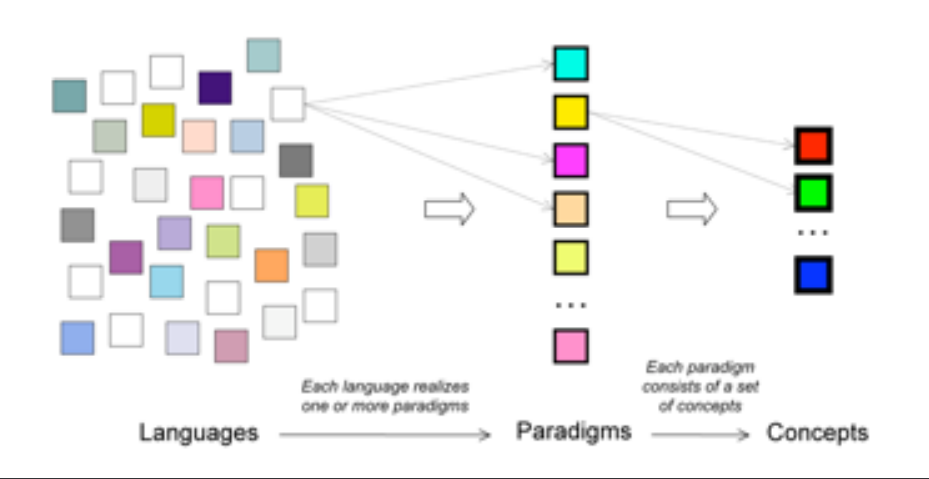
\includegraphics[scale=0.75]{Capture.PNG}
			%\caption{Légende de l'image}
		\end{figure}
		\item[* ] Une langue peut réaliser un
		paradigme : les langues "pures.
		\item[* ] La plupart des langages permettent plusieurs
		paradigmes.
		\item[* ] Certains langages sont conçus
		pour réaliser plusieurs paradigmes :
		les langages multi-paradigmes.
		\item[* ] Un langage peut évoluer et
		réaliser de nouveaux paradigmes.
	\end{itemize}
\subsection{Ceux qu'il faut connaître}
\begin{itemize}
	\item[* ] Impératif : spécifie les instructions au programme (pour arriver à un résultat)
	\begin{itemize}
		\item[* ] Programmation structurée : utilise un flux de contrôle structuré (conditions, boucles).
		\begin{itemize}
			\item[* ] Programmation procédurale : utilise des procédures pour structurer le programme.	
		\end{itemize}
		
		\item[* ] Programmation orientée objet : concept d'objets (données + code)
	\end{itemize}
\item[* ] Déclarative : spécifie le résultat au programme (pas les instructions)
\begin{itemize}
	\item[* ] Programmation fonctionnelle : un programme est une composition de fonctions.
	\item[* ] Logique : expression en termes de formules logiques.
\end{itemize}
\end{itemize}
\subsection{Règles générales pour un code propre}
\begin{itemize}
	\item[* ] Nécessité de normes de codage :
	\begin{itemize}
		\item[* ] Uniformisation des codes écrits par différents développeurs.
		\item[* ] Améliore la lisibilité
		\item[* ] Améliore la maintenabilité
		\item[* ]  Améliore la réutilisation
		\item[* ] (Peut) réduire la complexité
		
	\end{itemize}
\end{itemize}
\subsection{Développement piloté par les tests}
\begin{itemize}
	\item[* ] 3 lois (de Robert Martin) :
	\begin{itemize}
		\item[* ] Vous ne pouvez pas écrire de code de production avant d'avoir écrit un test unitaire défaillant (test unitaire
		d'abord)
		\item[* ] Vous ne pouvez pas écrire plus d'un test unitaire que ce qui est suffisant pour échouer, et ne pas compiler est un échec (un seul test unitaire échoué à la fois).
		\item[* ] Vous ne pouvez pas écrire plus de code de production qu'il n'est suffisant pour passer le test en cours d'échec (le code ne doit résoudre que le test unitaire)
	\end{itemize}
\item[* ] Un concept par test.
\item[* ] Répétable.
\item[* ] 5 étapes pour ajouter une nouvelle fonctionnalité :\\
\begin{itemize}
	\item[* ] Ajoutez un test qui passera si et seulement si l'exigence donnée est satisfaite.
	\item[* ] Exécuter tous les tests. Le nouveau test devrait échouer car la fonctionnalité n'a pas encore été implémentée.
	\item[* ] Ajoutez la quantité minimale de code pour réussir le test.
	\item[* ] Vérifier que tous les tests (y compris les précédents) passent.
	\item[* ] Refactoriser pour améliorer la lisibilité et la maintenabilité.
		\begin{figure}[!hbtp]
		\centering
		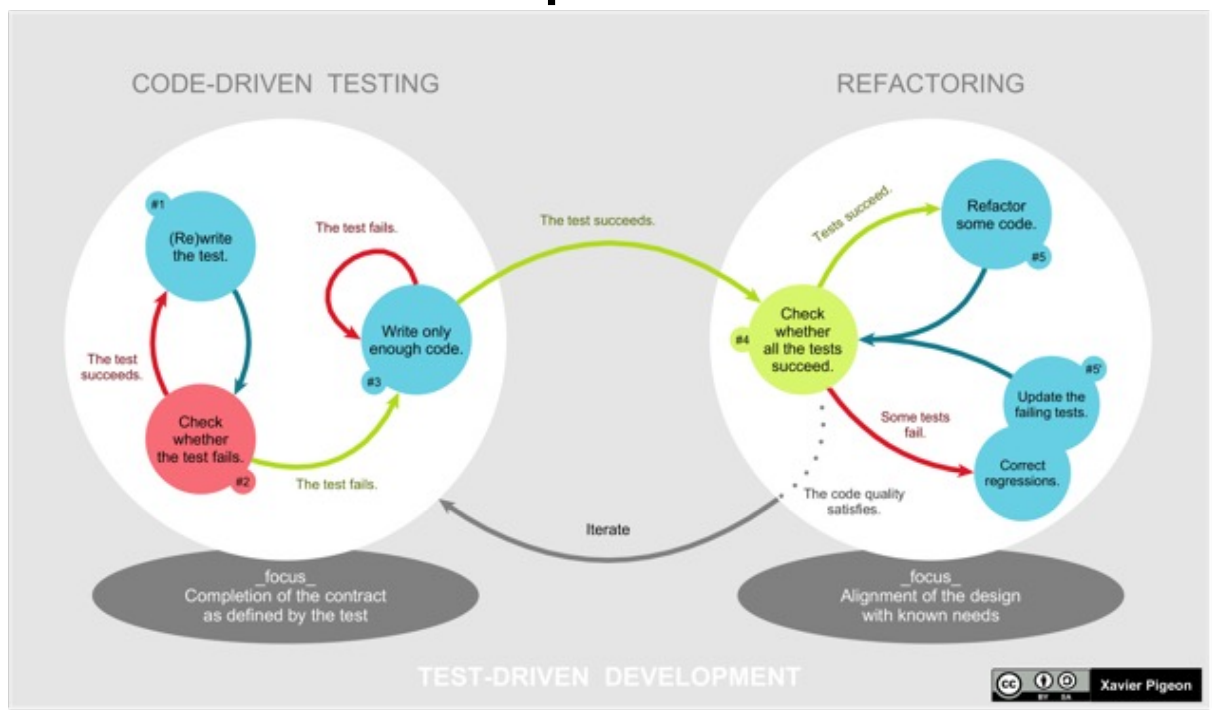
\includegraphics[scale=0.75]{Capture1.PNG}
		%\caption{Légende de l'image}
	\end{figure}
\end{itemize}
\end{itemize}
\end{document}